\chapter{Analyse de la méthode JFNK dans CEDRE}

  \paragraph{}
  In a previous chapter, we identified some methods from the literature that we wanted to use in our solver CEDRE, and some others from CEDRE that we wanted to improve.
  In another chapter, we discussed the practical implementation of said methods in the solver.
  The goal of this chapter is now to test those methods on several applications to comment on the choices we made.
  We need to define test cases that represent well enough target applications so we can comment on the performances of our choices.


  \section{Comparaison entre la matrice jacobienne explicite et la formulation sans matrice}

    \paragraph{}
    From our analysis and implementation, the main addition to the solver is the Jacobian Free Newton--Krylov method, and in particular the matrix-free approach.
    In this part, we will then compare two methods: the traditional method and the new one that uses the matrix-free approach.
    As we are interested in implicit time integration, we will use the implicit Euler method, for reasons previously discussed.
    The traditional method linearises the equation that the implicit Euler method produces, approximates the Jacobian matrix using the Jacobian matrix of the corresponding first-order scheme, and then solves the linear system with the Krylov subspace method GMRES.
    As we want to understand the impact of a better Jacobian matrix, we are only going to change how it is computed.
    The new method will then work in a similar way, except the matrix used in the linear solver is not actually computed, but the matrix-vector products are approximated using equation (\ref{eq:matrix_free}).


    \subsection{Turbulent transonic airfoil}

      \subsubsection{Definition of the test case}


        \PS{TODO: sûr de aoa et Re ?}

        \paragraph{}
        Our first application is a typical aerodynamics test case.
        It is a 2D simulation of the flow around an RAE 2822 wing profile.
        The only fluid is standard air.
        The Mach number is taken equal to 0.75, the chord is equal to $1\si{\meter}$, the angle of attack is $0\si{\degree}$ and we use the atmospheric conditions at 10km.
        This gives a Reynolds number of \num{6.3e6}.

        \paragraph{}
        We decided to use this first test case for multiple reasons.
        Firstly, it is a simple case in the field of computational fluid dynamics.
        It is a standard aerodynamics case, with a small mesh in comparison to many other 3D cases.
        This allows us to test out methods inexpensively.
        Secondly, this case belongs to the tutorial suite of our solver.
        It means that it is already well mastered by the team.
        Thirdly, even if it is only a standard aerodynamics case it still has some stiff features, such as turbulence modelling and a shock.
        Finally, it is a standard test case for turbulence modelling validation.
        Therefore there are many references in the literature using this case. \PS{LES DONNER !}
        Even if this thesis aims at multiphysics, it is often good to start slow, and that is what we are doing with this test case.

        \paragraph{}
        The mesh used for this simulation is an unstructured hybrid mesh made of triangles and quadrangles \PS{c'est bien ça ?}.
        Parts of it can be seen in figure \ref{fig:rae_mesh}.
        Cell sizes range from $2.5\si{\meter}$ far from the airfoil and $100\si{\micro\meter}$ at the wall.
        At the wall, there is a C-shaped layer of regular cells.
        This helps better capture boundary layer effects near the profile and the \PS{pas vraiment lâcher tourbillonnaire}.
        Also, at those conditions, a shock is expected to develop on the upper part \PS{extrados ?}.
        Special treatment such as refinement was applied to the mesh at the expected shock location.

        \begin{figure}
          \centering
          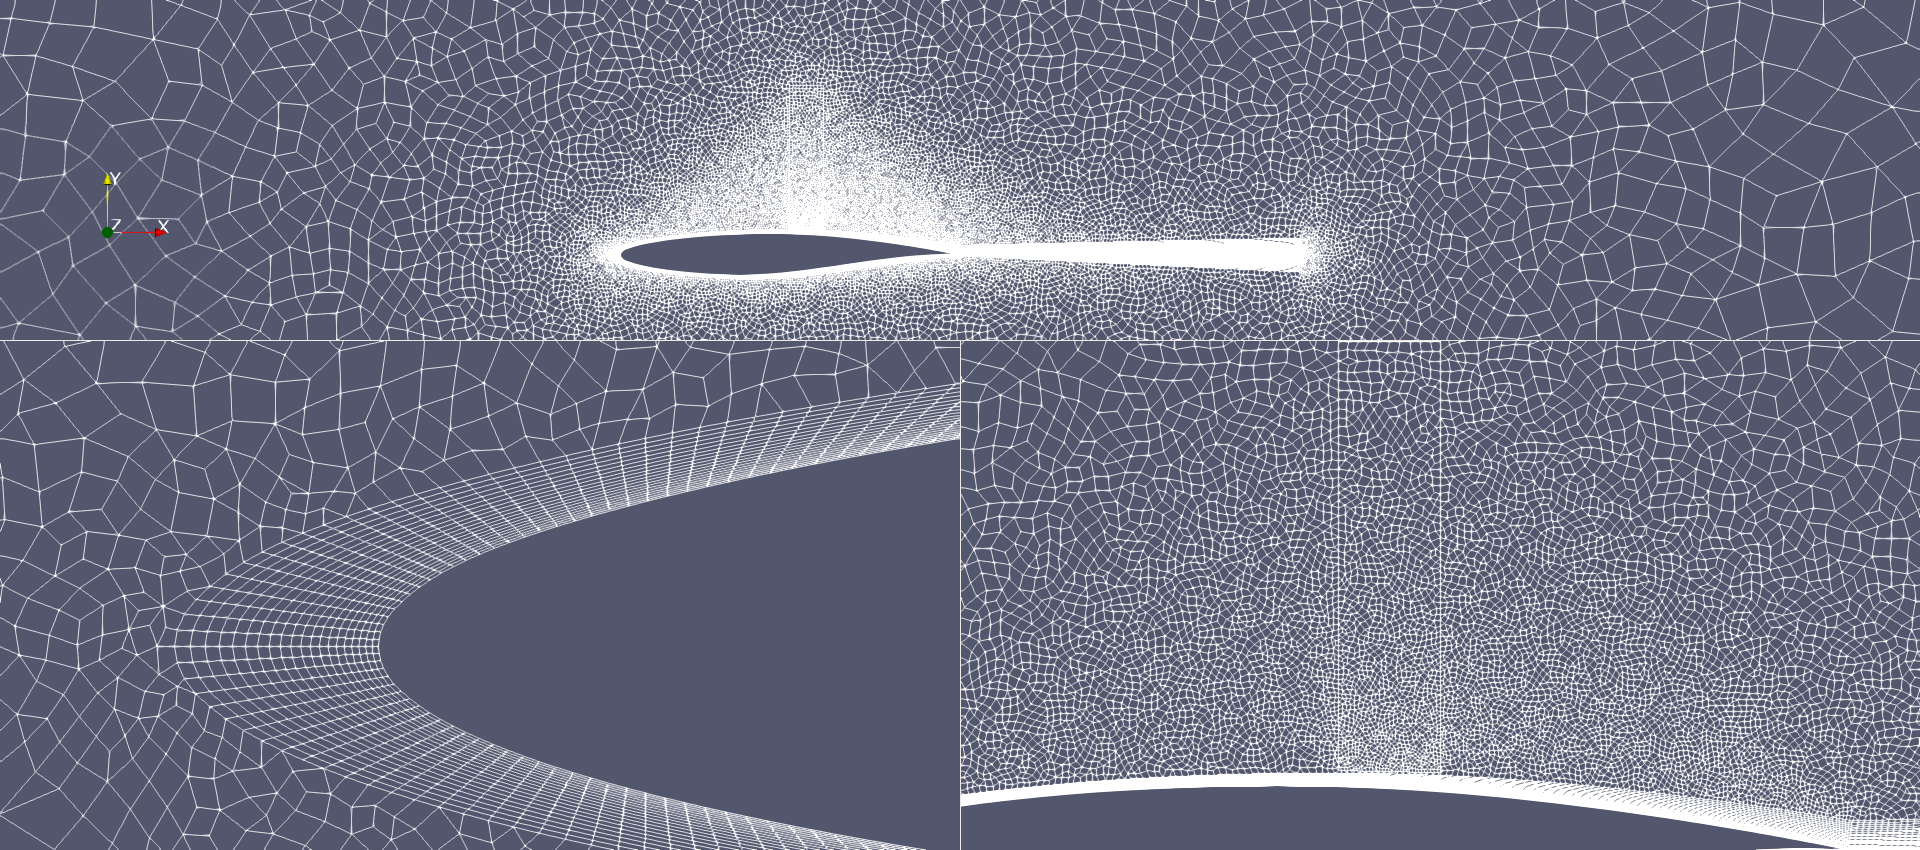
\includegraphics[width=\textwidth]{figures/rae_mesh.png}
          \caption{Mesh for the RAE 2822 test case. Close up on the expected shock location and the wall on the leading edge.}
          \label{fig:rae_mesh}
        \end{figure}

        \paragraph{}
        The model used is the Reynolds Averaged Navier--Stokes equations, or RANS.
        Simply put, every scale of the turbulence is modelled \PS{c'est bien ça ?}.
        For this case, we decided to use the famous Spalart--Allmaras turbulence model.
        It is well known for being one of the simplest turbulence models, which is fine for us as we want to set up a simple first test case.
        The spatial discretisation method is a second-order Finite Volume method, using the HLLC Riemann solver and Multislope method with a Van--Leer slope limiter.
        We also use local time stepping to speed up the convergence.

        \PS{Note pour moi même: est-ce que je refais JFNK ordre 1 pour montrer qu'on retrouve la méthode classique ? Sauf que vu qu'il y a la turbulence j'en suis pas certain, mais ça montrerai que c'est bien sur deux points de vue (tout les modèles + discrétisation spatiale) donc oui fais le }

      \subsubsection{Analysis of the results}

        \PS{Figure champ (mach)}

        \PS{Figure CP comparative}

        \PS{Qu'est-ce qu'on peut regarder pour avoir une différence, flux de chaleur ?}

        \paragraph{}
        We are now going to compare the results from the two different simulations.
        It is first worth noting that before trying the JFNK method, we need to start the computation using the traditional method.
        We assume that because of the matrix-free approximation, it is less robust at the beginning.
        Only some iterations are needed, just to start the development of start the no-slip boundary layer.
        After that, we can restart the computation with the traditional method on one side and with the new method on the other.

        \begin{figure}
          \centering
          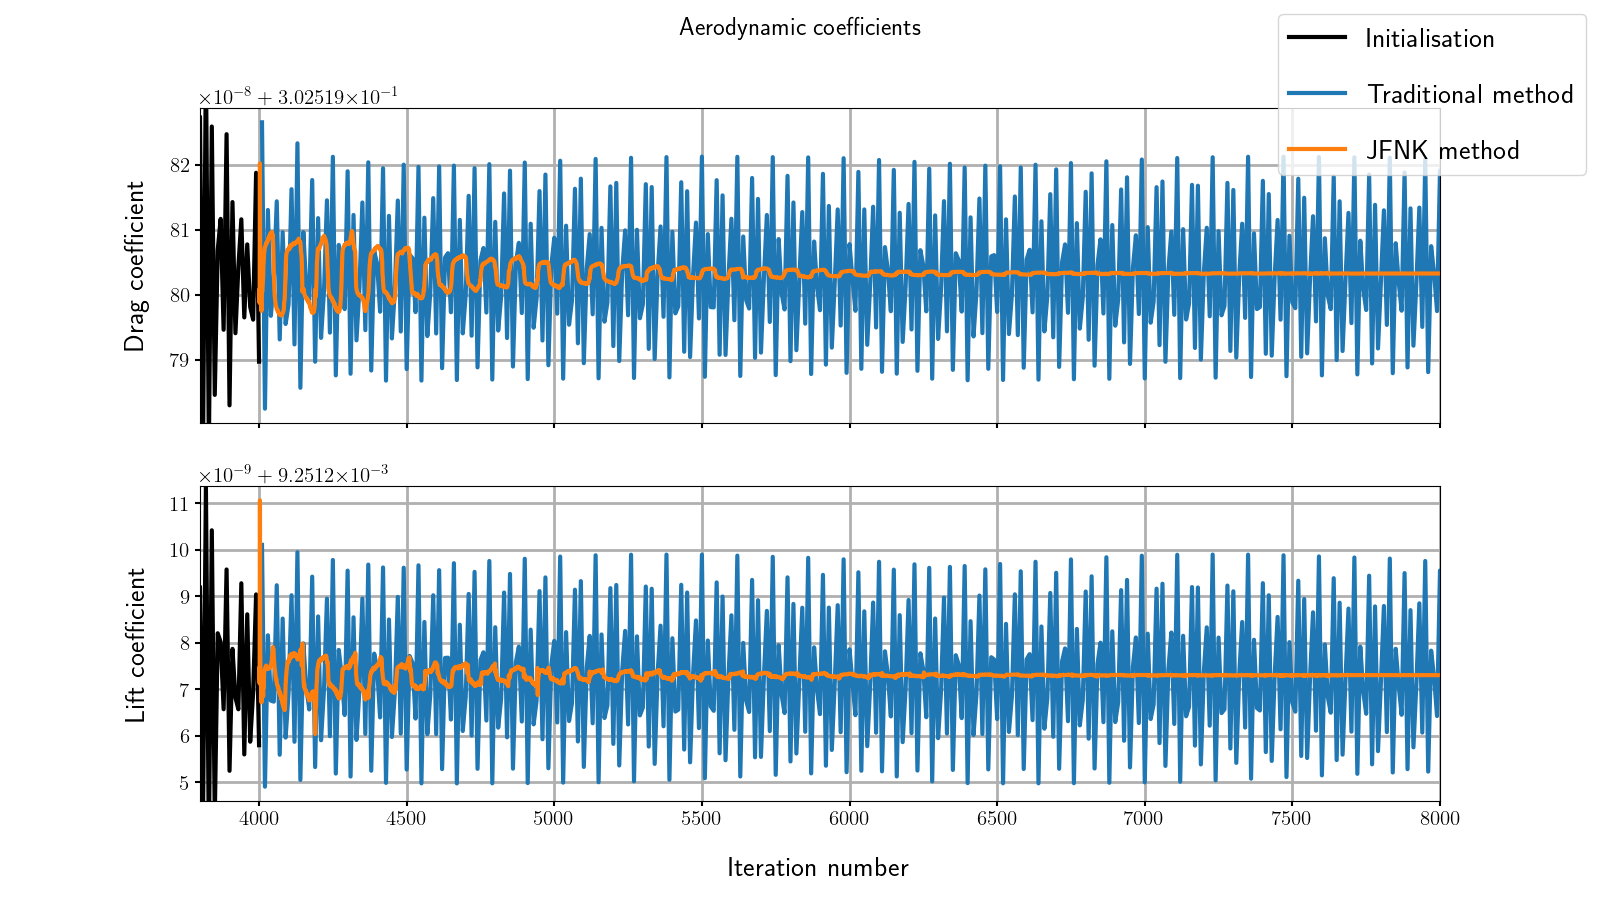
\includegraphics[width=\textwidth]{figures/rae_coefficients.png}
          \caption{\PS{TODO: Aerodynamic coefficients (lift and drag) for the profile throughout the computation.}}
          \label{fig:rae_coefficients}
        \end{figure}

        \paragraph{}
        We can first look at a global image of the flow.
        This is done in figure \PS{TODO} where we can look at the pressure field near the airfoil.
        In particular, as expected, we see the shock on the upper part.
        The two computations give similar results: they are indistinguishable by just looking at the pressure field.
        This is to be expected as the traditional method gives already satisfying results on such applications.
        We can also look at the pressure coefficient around the airfoil in figure \PS{TODO}.
        Once again, the two curves are indistinguishable.
        Finally, we can look at the aerodynamic coefficients, the drag and lift coefficients, throughout the simulation in figure \ref{fig:rae_coefficients}.
        This time, we see an improvement from our method: the coefficients are much more stable, which means the convergence is better with our method.

        \paragraph{}
        In order to find out if our method did help the convergence of the solver, we need to look at the residuals.
        To define the residuals, we need to go back to the partial differential equation (\ref{eq:pde}) from which we started.
        The residual is in fact the value of the function $\operatorname{F}$ from this equation.
        We can then understand its name for steady problems: it is what is left and still needs to be removed to find a steady solution.
        To decide on the convergence of a steady simulation, we look at this residual norm throughout the computational domain $\mathcal{D}$.
        More precisely, we look at this residual component by component.
        For example, the residual 2-norm associated with the $i$th component is:
        \begin{equation}
          \norm[2]{\operatorname{F}_i} = \int_\mathcal{D} \left| \operatorname{F}_i \right| \mathrm{d}v
        \end{equation}
        and the $\infty$-norm is:
        \begin{equation}
          \norm[\infty]{\operatorname{F}_i} = \max_\mathcal{D} \left| \operatorname{F}_i \right|
        \end{equation}
        In this fluid dynamics application, we can look at the residual norm associated with the conservative variables: the density, the momentum components, the energy and the turbulent variable from the Spalart--Allmaras model $\nu_t$.

        \begin{figure}
          \centering
          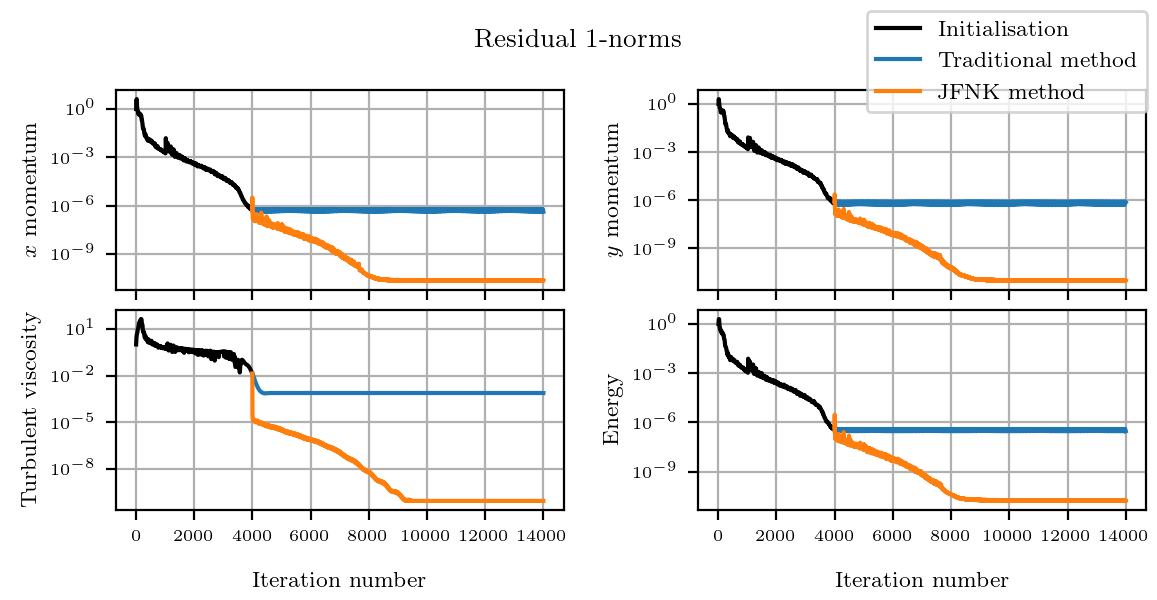
\includegraphics[width=\textwidth]{figures/rae_residuals.png}
          \caption{\PS{TODO: Residual norm for the turbulent viscosity throughout the computation.}}
          \label{fig:rae_residuals}
        \end{figure}

        \paragraph{}
        Figure \ref{fig:rae_residuals} shows the residual norms from our two computations.
        The gain from using the JFNK method appears clearly.
        The final residual norm is much smaller for each and every conservative component.
        This means that the Jacobian free Newton--Krylov method is able to reach a better convergence level than the traditional method.
        In other words, the better Jacobian matrix approximation from our new method leads to a better convergence than the older poor approximation.
        \PS{Que dire de plus ?}

        \paragraph{}
        In this first test case, we looked at the residual norms as the fields computed by both methods were almost identical.
        Moreover, our method was even able to reach better convergence levels.
        This validates our method on a first simple case, albeit with turbulence modelling and a shock.


    \subsection{Hypersonic reactive sphere}

      \paragraph{}
      The second application we selected to compare the Jacobian Free Newton--Krylov with the traditional one is the computation of the flow around a hypersonic solid sphere.
      Because of the high energy of the surrounding flow, the air molecules can separate and even form a plasma \PS{check traduction}.
      The hypersonic reactive sphere is a well-known case, for both experimental \cite{Lobb1964} and numerical studies \cite{DobrovGimadievKarpenkoEtAl2022}.
      This is a simple yet representative test case of CEDRE applications.
      It then makes a lot of sense to analyse our new method on it.

      \subsubsection{Definition of the test case}

        \PS{AVEC OU SANS CHIMIE ?}

        \begin{figure}
          \centering
          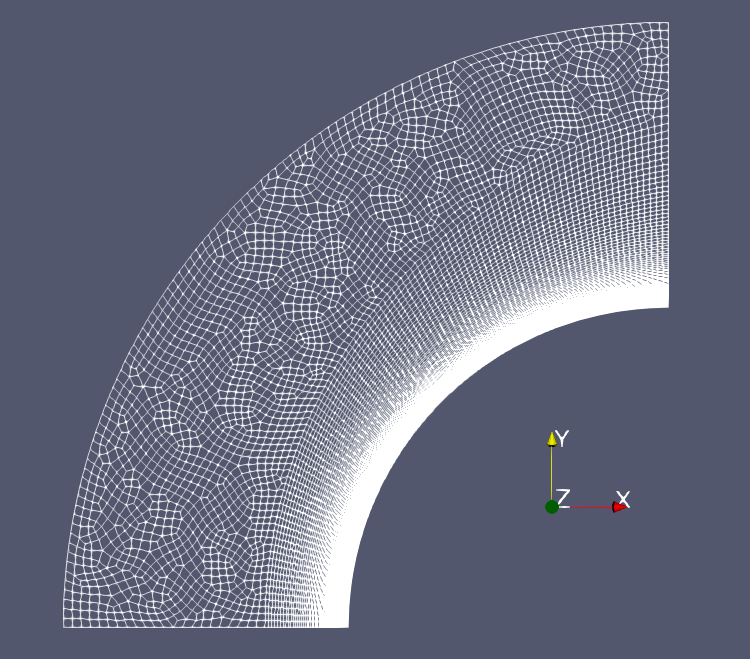
\includegraphics[width=0.6\textwidth]{figures/sphere_mesh.png}
          \caption{\PS{TODO: c'est pas le bon maillage}}
          \label{fig:sphere_mesh}
        \end{figure}

        \paragraph{}
        The 2D mesh is shown in figure \ref{fig:sphere_mesh}.
        It is a regular mesh made of quadrangles, with refinement in the radial direction at the wall boundary and at the expected shock location.
        The refinement at the wall boundary helps to compute more precisely the physical phenomena that happen at said boundary.
        The refinement at the shock is a requirement of the spatial discretisation methods.
        In order to get a clean and slim shock, the cells near the shock must have a high aspect ratio.
        Otherwise, artificial vorticity is created when going through the shock, which will give wrong results downstream. \PS{c'est bien pour ça ?}
        This expected shock location is obtained from a previous computation, made with a coarser mesh.
        This mesh is used in a 2D axisymmetric computation to get the flow around a 3D solid sphere.

        \paragraph{}
        The solid sphere is modelled by an isothermal wall boundary condition.
        This is a representative choice as well, as the heat flux going through the wall is one of the main interests of such computation.
        Moreover, as it depends on the derivatives of the flow variables, it is usually harder to get a correct value for the heat transfer.
        A better convergence will lead to better derivatives, which will lead to better physical results for such case users.
        No turbulence model is used, as the flow is mostly laminar.

        \paragraph{}
        \PS{KEX vs MTP}

        \paragraph{}
        The main feature of this test case is that it simulates a hypersonic flow.
        At the left, the input boundary condition feeds air at Mach 15.
        This will induce a strong shock, meaning a strong discontinuity in the flow.
        As this is a typical application of our solver, it is of importance to us that the new method behaves well with such flow features.
        When going through a strong shock, the temperature of the flow will increase a lot.
        The flow is made of air, or a mixture of 77\% \ce{N_2} and 23\% \ce{O_2}.
        At the high temperature they reach after the shock, the molecules can decompose into \ce{N}, \ce{O}, and \ce{NO}.
        They can even get ionised.
        In our model, we end up using 11 possible species: \ce{N_2}, \ce{O_2}, \ce{N}, \ce{O} and \ce{NO}, the corresponding cations \ce{N_2^+}, \ce{O_2^+}, \ce{N^+}, \ce{O^+} and \ce{NO^+} and the electrons \ce{e^-}.

        \paragraph{}
        This test case is a typical application of CEDRE, as opposed to the previous one which focuses more on the aerodynamic properties.
        Indeed CEDRE does not try to be a pure aerodynamic solver but a multiphysics one, equipped to solve high-energy problems.
        Reentry phenomena are therefore in the scope of our solver.
        Any improvements coming from our method on such applications would benefit a lot of CEDRE users on their applications.


      \subsubsection{Analysis of the results}

        \paragraph{}
        Once again, a first computaiton is done using the more robust traditional method.
        Indeed, the flow in the first cell against the sphere and the symmetry axis is initialised with a Mach number of 15 going straight into the wall.
        The matrix-free approximation struggles with such stiff initialisations, which is why we must start the computation with another method, just until the shock has started to detach from the wall.
        Practically this amount to just a few iteration, compared to the number required to achieve convergence.

        \paragraph{}
        We first look at the different fields from the two computations.
        Once again they are similar and we will use the residuals to compare them, but we can check we are indeed computing the features of interest.
        In figure \PS{TODO}, we see that the shock is present and that it falls as expected in the refined region.
        We see in figure \PS{TODO} the mass fraction of the various species downstream of the shock, which means we are actively computing the chemical features of the flow, as expected.
        \PS{Comparaison distance corps shock avec \cite{Lobb1964} ?}

        \paragraph{}
        Once again, we will not see any difference between the two results if we look at the \PS{standard} quantities.
        We might see them if we look at quantities that depend on the derivatives of the flow variables, and that is why we will look at the \PS{heat transfer coefficient} at the wall.
        The results are displayed in figure \PS{TODO}.
        \PS{A VERIFIER MAIS DE MEMOIRE :}
        Unfortunately, there is not much difference to be seen between the two methods: they both produce the same heat transfer coefficient.
        We also see an issue: the heat flux should be maximum at the stagnation point, but we see in figure \PS{TODO} that it is not, and the slope of the heat transfer coefficient is not null at the stagnation point in both of our simulations.
        This shows an inaccuracy of the solver.
        However, as we will show next, the time integration is able to find the correct converged steady solution.
        Therefore this inaccuracy comes from the spatial discretisation method.
        The results are not accurate from a physical analysis perspective, but for us, the methods both work fine: they find the expected steady solution, albeit it is not the expected physical one.

        \paragraph{}
        The advantage of the new method appears when we look at the residuals: we see in figure \PS{TODO} that the new method gives a better convergence.
        The difference between the traditional method and the new one is that the traditional method uses the Jacobian matrix of the first-order spatial discretisation method, whereas the new one approximates the true Jacobian matrix using the approximation (\ref{eq:matrix_free}).
        We decided to test this.
        If we use the approximation (\ref{eq:matrix_free}), but using the first order evaluation of $f$, then we should get the same Jacobian matrix as the one used by the traditional method.
        We look at the residual norms from this method, which we can call the first-order JFNK method, and we see in figure \PS{TODO} that it is indistinguishable from the residual norms from the traditional method.
        It first validates the development of the matrix-free approximation.
        It also confirms that the traditional method uses the Jacobian matrix of the first-order spatial discretisation method.
        Finally, it validates the choice of $\varepsilon$ and the matrix-free approximation, as it is able to give the same result as when we use the Jacobian matrix.
        When we use the new method, using the true function $f$ with a second-order, we see that we can get a much smaller residual norm.
        It confirms that using a better Jacobian matrix helps the overall convergence when solving steady problems.


    \paragraph{}
    In a previous part we suggested that the poor quality of the Jacobian matrix used in our solver was an obstacle to achieve good convergence.
    We then proposed an improvement: the Jacobian Free Newton--Krylov method using the matrix-free approximation (\ref{eq:matrix_free}).
    We compared this new method with the traditional one on two simple yet representative application of our solver.
    This comparaison showed that indeed, using a better Jacobian matrix lead to lower residual norm.
    The new method can be usefull when looking at quantities that require precise convergence, for instance the derivatives of the flow variables.
    However, the main drawback of this new method is its computational cost.
    This cost is not inherent to the method, but comes from our solver properties as was discussed previously.
    The recommended usage is then to start a computation using the inexpensive traditional method, and then achieve better convergence using the more precise yet more expensive new method.


  \section{Utilisation de la formulation sans matrice sur un nouveau modèle de fluide}
    \subsection{Modèle Multi-températures}
    \subsection{Sphère hypersonique}
      \subsubsection{Modèle réactif complet}
      \subsubsection{Modèle réactif simplifié}
